\section*{Descripción}

En la presente investigación, se compara el desempeño de dos algoritmos de reducción de dimensionalidad para resolver un problema de clasificación.

\textbf{Algoritmo 1}: Entrenar \textbf{por separado} un \textit{Autoencoder Undercomplete} $(g \circ f_1)(x)$ y una red neuronal $(h_1 \circ f_1)(\bm{x})$ totalmente conectada que cuyas primeras capas están definidas por el \textit{encoder} $f_1(\bm{x})$ con sus pesos congelados.

\textbf{Algoritmo 2}: Entrenar \textbf{simultaneamente} una red neuronal $(h_2 \circ f_2)(\bm{x})$ totalmente conectada cuyas primeras capas aprendan una representación de menor dimensionalidad.

\textbf{Problema de clasificación}: Clasificar \textit{tweets} como tóxicos o no tóxicos. Los datos utilizados fueron publicados para una competencia de \textit{Kaggle} \cite{jigsaw-toxic-comment-classification-challenge} organizada por \textit{Jigsaw}: ``una unidad de Google que explora las amenazas a las sociedades abiertas y crea tecnología que inspira soluciones escalables''.

En \ref{fig:autoencoder} se presenta una arquitectura estándar de un \textit{Autoencoder Undercomplete}. Consiste en una red neuronal artificial totalmente conectada que es entrenada para codificar la entrada $\mathbf{X}$ a una representación de menor dimensionalidad mediante el \textit{encoder} $f_1$ y luego reconstruir $\mathbf{X}$ minimizando una función de pérdida $\ell(\bm{x},g(f_1(\bm{x})))$ como la pérdida cuadrática que penaliza $g(f_1(\bm{x}))$ en función de cuánto difere con $\bm{x}$.

Como en el contexto de aprendizaje supervisado la tarea es conseguir una hipótesis $h_1$ que permita \textit{mapear} desde un conjunto de entrada $\mathcal{X}$ hacia un conjunto de salida $\mathcal{Y}$, una vez entrenado el \textit{Autoencoder} $(g \circ f_1)(x)$ se utiliza el \textit{encoder} $f_1$ para codificar las entradas a un nuevo modelo $h_{1}$. 

\begin{figure}[h]
\centering
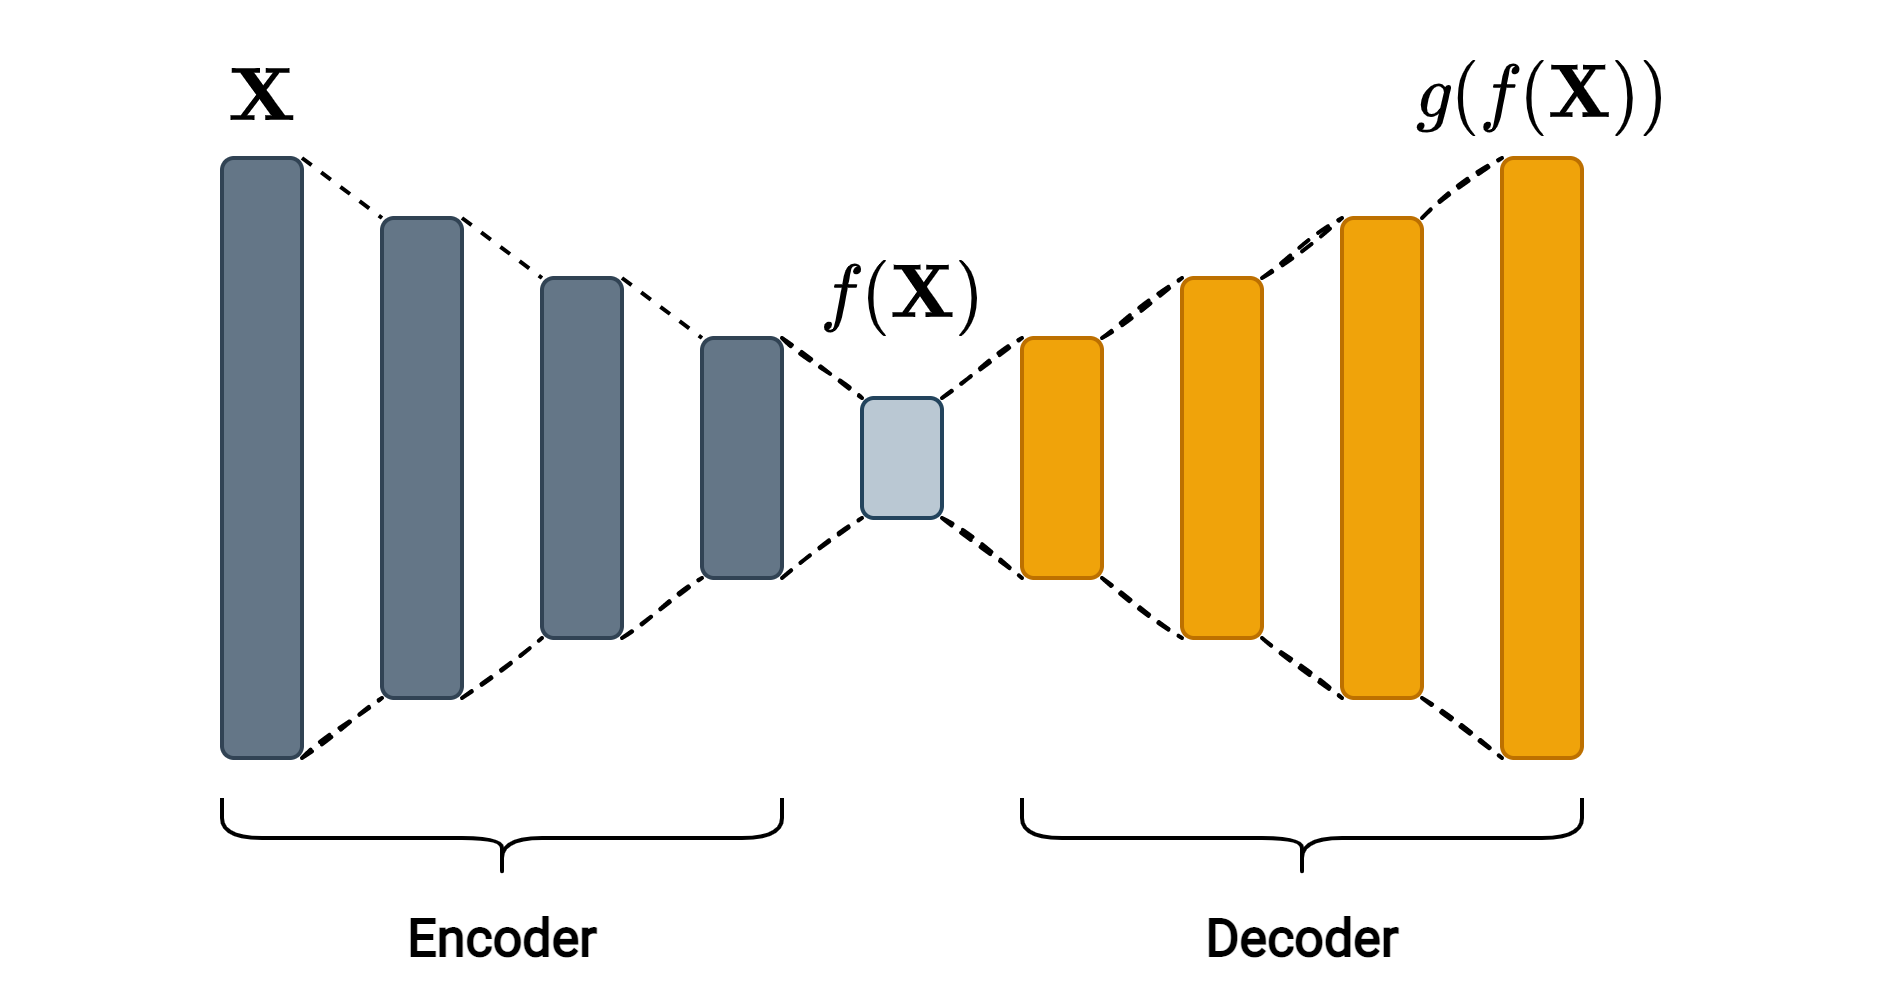
\includegraphics[width=0.4\textwidth]{autoencoder}
\caption{\label{fig:autoencoder} \textit{Autoencoder Undercomplete}}
\end{figure}


En \ref{fig:fish} se presenta la arquitectura neuronal \textbf{Fish} propuesta. Consiste en una clásica red neuronal artificial totalmente conectada que es entrenada para aprender \textbf{simultaneamente} la codificación \textit{ad-hoc} $f_2$ y la tarea supervisada $h_2\colon \mathcal{X} \rightarrow \mathcal{Y}$ . Primero, sus primeras capas se encogen para lograr una representación de menor dimensionalidad; Segundo, una capa expande esta representación; Tercero, las siguientes capas se encogen hasta la capa de salida.

\begin{figure}[h]
\centering
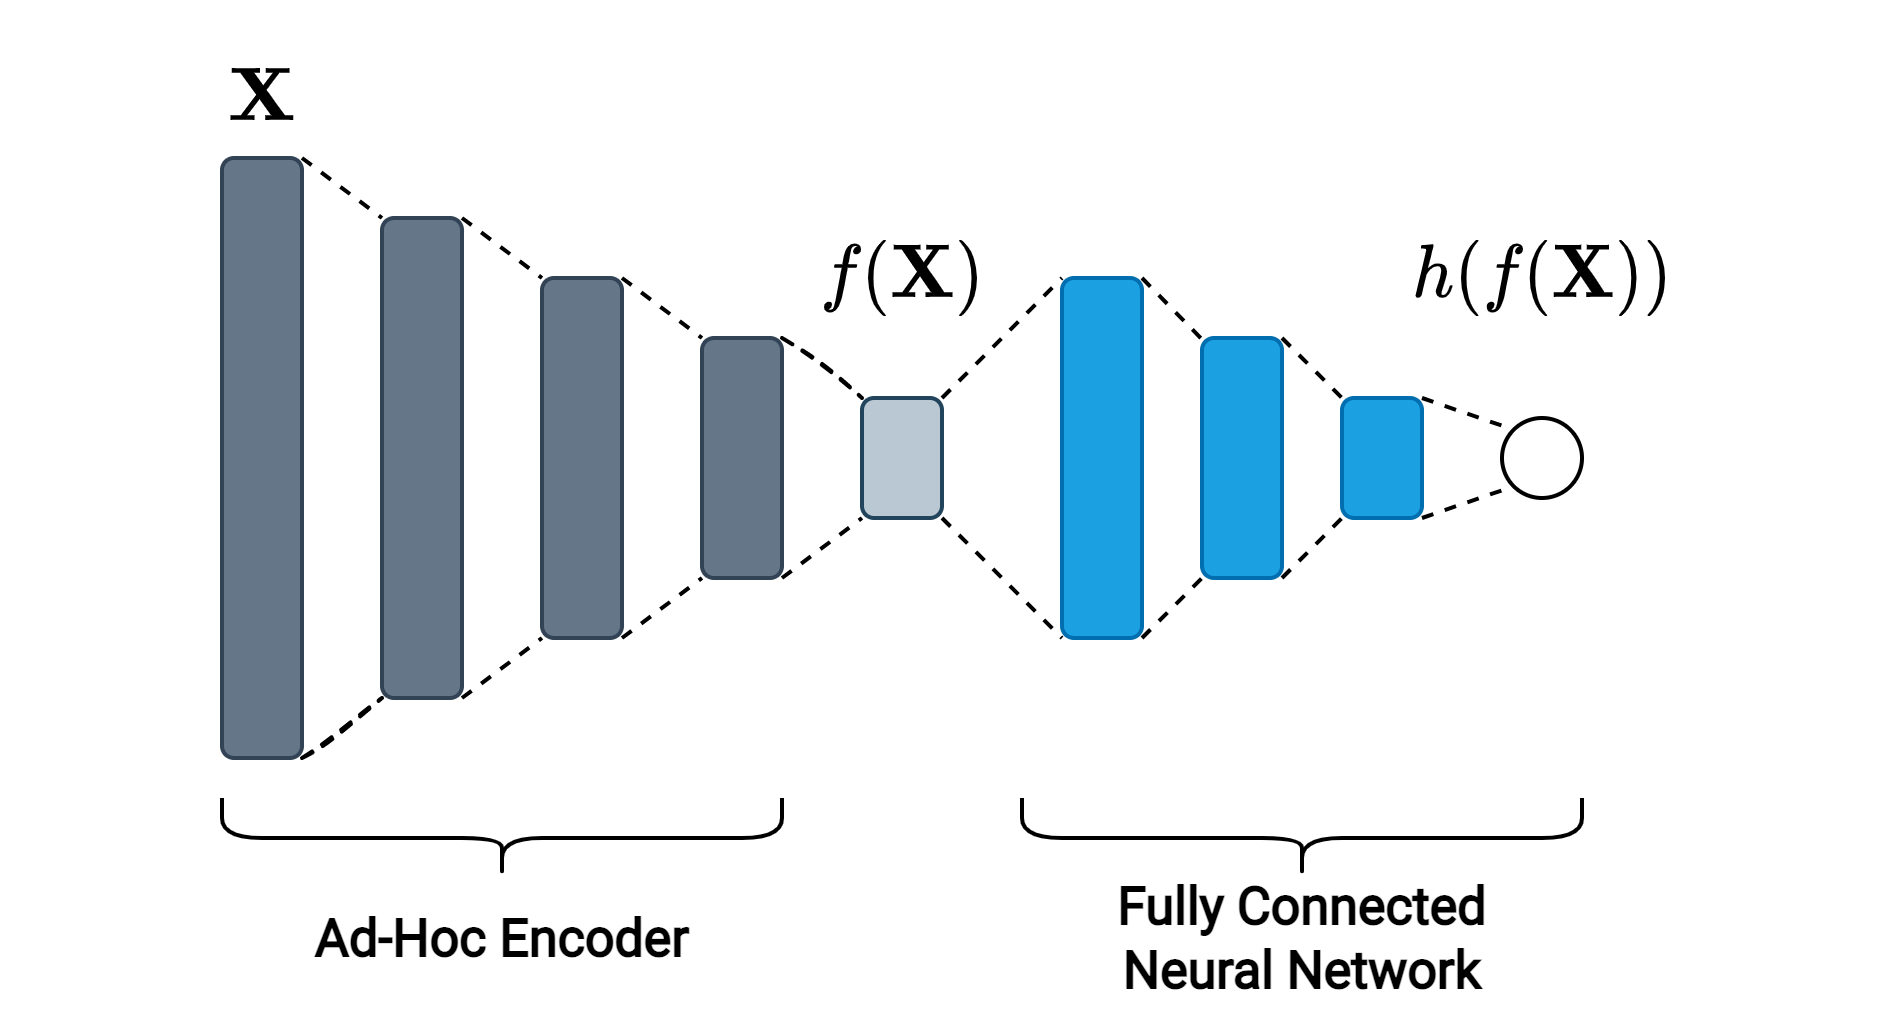
\includegraphics[width=0.45\textwidth]{fish}
\caption{\label{fig:fish} Red Neuronal Fish}
\end{figure}